\documentclass[hidelinks,a4paper, 12pt]{article}

\usepackage[top=0.5in, bottom=0.5in, left=0.9in,right=0.5in]{geometry}
\usepackage[T1]{fontenc}
\usepackage{hyperref}
\usepackage{graphicx,wrapfig}
\usepackage{enumitem}
\renewcommand{\arraystretch}{1.5}

%Font into Helvet
\renewcommand{\familydefault}{\sfdefault}
\usepackage{helvet}

\usepackage[absolute,overlay]{textpos}

%hyperlink
%\usepackage{hyperref}
\usepackage{xcolor}
\hypersetup{colorlinks=false,linkbordercolor=red,linkcolor=black,pdfborderstyle={/S/U/W 1}}

\begin{document}

%no page number
\pagestyle{empty}




\begin{wrapfigure}{r}{0.20\textwidth}
	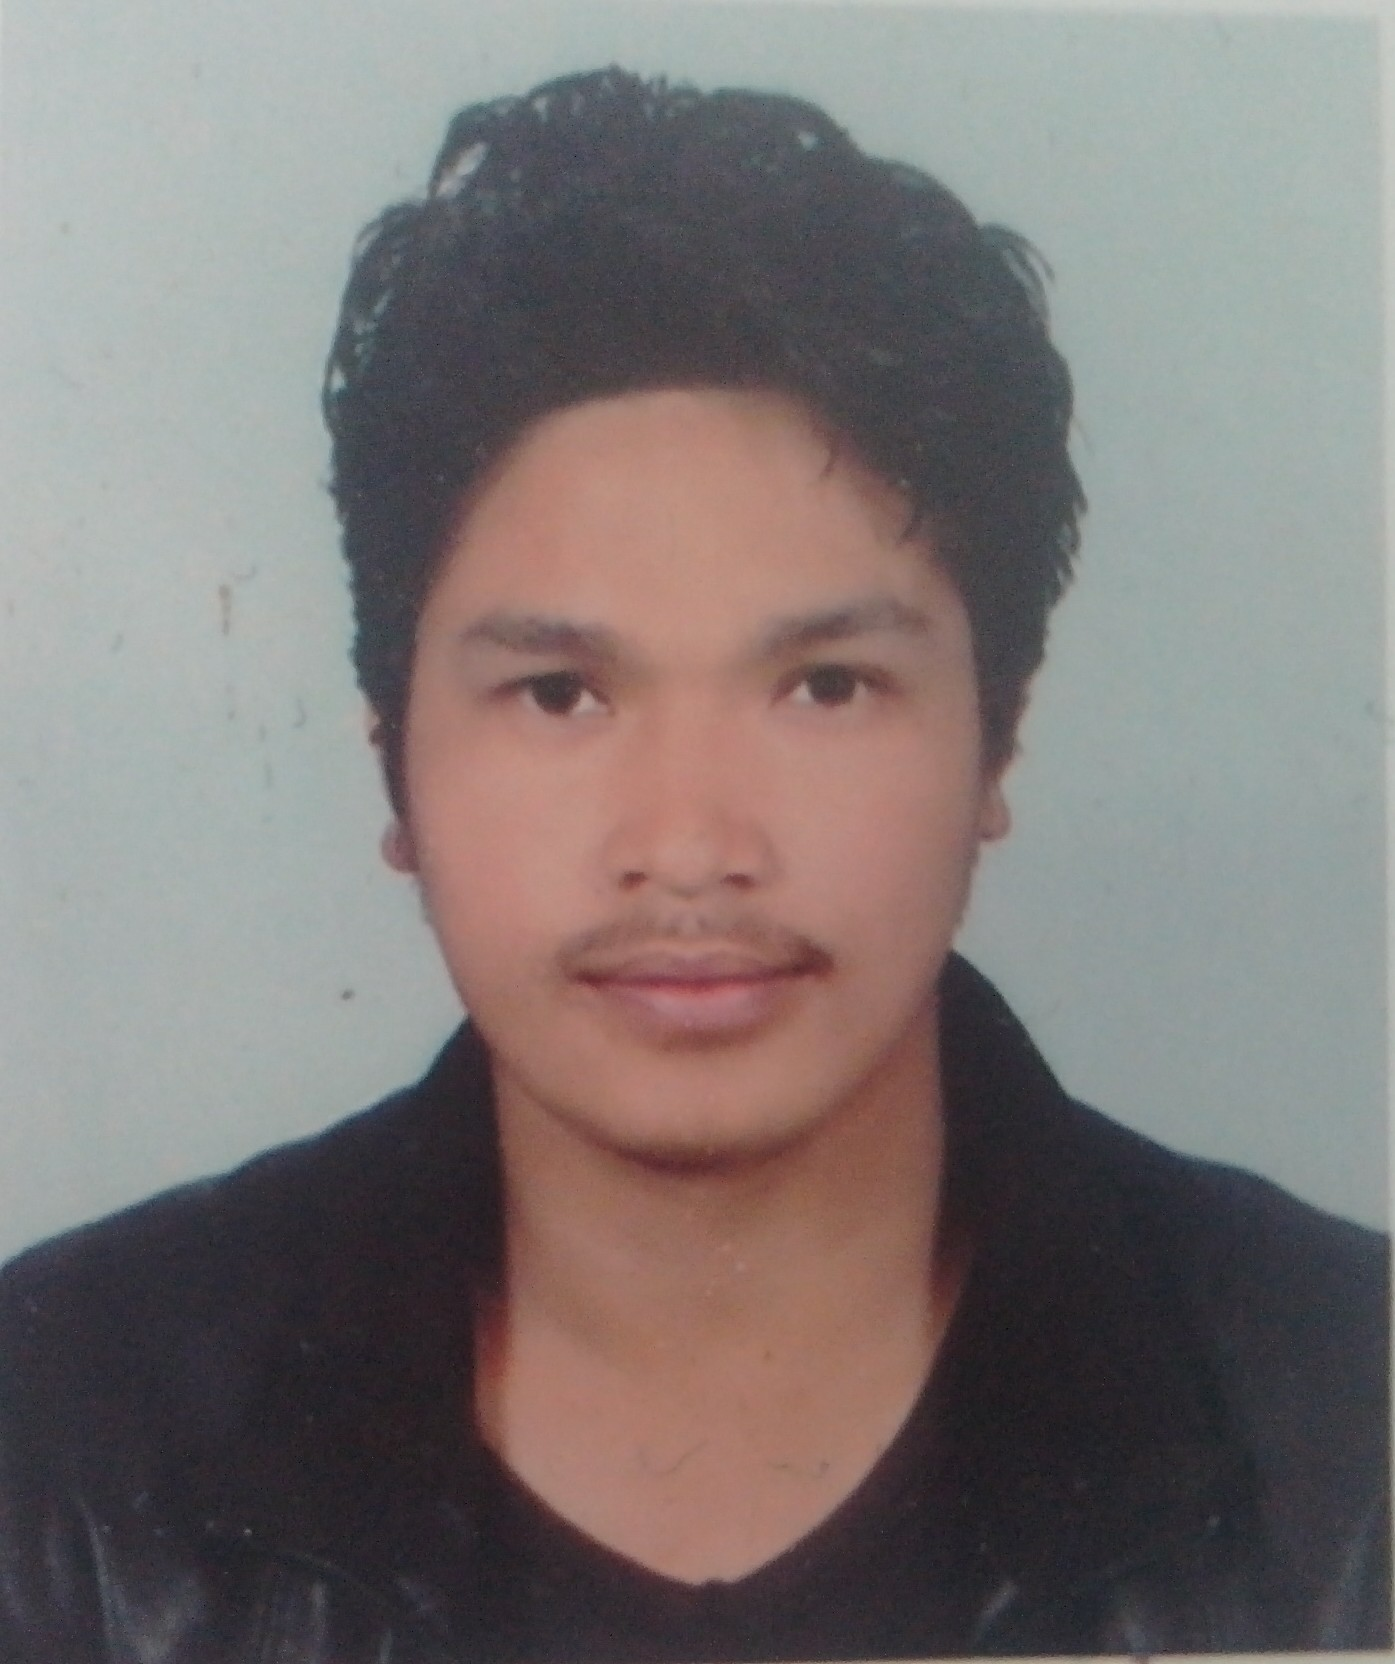
\includegraphics[height=1.20in, width=1.10in]{k}
\end{wrapfigure}
~
{\Huge
	\textbf{Kritish Pahi} \\}
	B.E. Computer Engineering\\
	{Mobile: 977-9849728755}\\
	{E-mail: kritishpahi@gmail.com}\\
\vspace{2.2mm}
	
%\begin{wrapfigure}{c}{0in}\end{wrapfigure}
 \rule[2pt]{0.9\textwidth}{1pt}
\vspace{1mm}

{ \Large \textbf{Personal Details:}\\
}
\begin{tabular}{l l}
	 \textbf{\emph{Name }} & : Kritish Pahi \\
	 \textbf{\emph{Address }}&  : Kamalbinayak 4, Bhaktapur \\
	 \textbf{\emph{Gender }} & : Male \\
	%\textbf{\emph{BloodGroup}} & : B +ve \\
	%\textbf{\emph{Marital Status }} & : Unmarried \\ 
	 %\textbf{\emph{Date of birth }} & : 29\textsuperscript{th} June 1995 \\ 
	 %\textbf{\emph{Religion }} & : Hinduism \\ 
	 \textbf{\emph{Driving Licence}} & : 2-Wheelers 
\end{tabular}
\vspace{8mm}

{\Large \textbf{Objective:} \\ 
}
To be an efficient Software Professional in an organization \& looking forward
to an opportunity where I can utilize my professional skills that offers 
challenges and professional growth while being resourceful, innovative 
and flexible.

\vspace{8mm}
{\Large \textbf{ Education Details: } \\
}
\begin{tabular}{l l l l}
	\textbf{Level} & \textbf{Institute} &\textbf{Year} & \textbf{Percentage} \\ \hline
	S.L.C & Prabhat English Higher Secondary School & 2011 & 88.0 \\ \hline
	H.S.E.B (Science) & Khwopa Higher Secondary School & 2013 & 82.40 \\ \hline
	B.E(Computer) & Institute of Engineering, Central Campus & 2013-Enrolling & - \\ \hline
\end{tabular}

\vspace{8mm}
{\Large \textbf{ Technical Profiles: } \\
}
\begin{tabular}{l l}
	\textbf{Languages:} & C, C++, HTML, PHP, CSS, Python, SQL, JavaScript \\
	\textbf{Operating System:} &  Linux, Windows \\
	\textbf{Application Packages:} & Office Packages, Vim, Latex \\ 
	\textbf{Framework: } & Bootstrap, Laravel, Django, JQuery \\
    \textbf{Database:} & MySQL, Mongodb, Postgresql
	
\end{tabular}

\vspace{8mm}
{\Large \textbf{Areas of Interest:} \\
}
\vspace{-5mm}
\begin{itemize}[noitemsep]
\addtolength{\leftskip}{8mm}	
    \item Machine Learning
	\item Software Development
	\item Computer Networks
	\item Web Development
	\item Mobile Application Development

\end{itemize}

\vspace{8mm}
{\Large \textbf{Personal Skills and Strengths:}\\
}
\vspace{-5mm}
\begin{itemize}[noitemsep]
\addtolength{\leftskip}{8mm}
	\item Quick Learner
	\item Leadership quality
	\item Ability to be a good team player
	\item Motivating and Convincing Power
	\item Good communication skill
\end{itemize}

\vspace{8mm}

{\Large \textbf{Projects Done:} \\
}
\vspace{-5mm}
\begin{itemize}

	\item \textbf{Pacman } \emph{(2014)} \\
		\small An old, classic and popular game with Artificial Intelligence
		chasing by the ghost. Also in two player mode. C++, SDL
	%\item \textbf{Multi-Security System} \emph{(2014)} \\
	%	\small A security system particularly designed for home application
	%	using laser sensor, step sensor to detect intruders. AVR 
	%	micro controller programming and interfacing
    \item \href{https://github.com/nac-gantabya/gantabya}{\textbf{Gantabya}} \emph{(2015)} \\
		\small A web-based as well as Android based application to recommend
		tourists about their destination based on their preference and budget
		plan. HTML, CSS, Bootstrap, PHP, MySQL
	%\item \textbf{Hangman} \emph{(2015)} \\
		%\small Popular game among the students, guessing letters for the 
		%words. Python
    \item \href{https://github.com/kritishpahi/SoftwareEngineering}{\textbf{Alumni Database Management} }\emph{(2015)}
		\small. Web based application for academic institutes to keep 
		track of Alumni of the institutes. PHP, MySQL, Laravel
    \item \href{https://github.com/kritishpahi/EduSpace}{\textbf{EduSpace}} \emph{(2016)} \\
		\small Django based website to helps students learn theories with
		their simulations and praticals. Python, Bootstrap, Django
    %\item \textbf{Departmental Store Management} \emph{(2016)}
	%	\small Simple management of products, orders, suppliers in
	%	Departmental Store and mainly a website to prepare bills for 
	%	the goods purchased by customers. Python, Bootstrap, Django
%    \item \href{https://github.com/kritishpahi/AnswerBot}{\textbf{AnswerBot}}\emph{(2016)}
%		\small A bot to answer to WH-question and to interact with human
%		using Natual Language Processing. Python, Wiki-scraping, NER
\end{itemize}

\vspace{8mm}
{\Large \textbf{ Training and Achievements: }\\ }
%\large \textbf{Training}
\vspace{-5mm}
\begin{itemize}
	\item  Participated in Crash Courses on AVR Training (2014), Windows 
	App Development (2014)
	\item 3rd Prize Winner in LOCUS-2014 Theme based Hardware Category 
	\emph{Multi-Security System}
	\item Ncell App camp 2015 with Top 150 ideas. \emph{Gantabya}
	%\item Participation in LOCUS 2014, 2015, 2016 National Technical Fest. 
	\item Participated in Crash Course on NodeJs(2016), Mongo DB (2016) 
	%\item Participated in two days \emph{Make \& Learn } Robotic Workshop
    \item Two weeks Internship in \emph{Wireless Service Directorate} in Nepal Telecom (2016).
\end{itemize}

\vspace{5mm}

{\Large \textbf{Minor Project: }\\}
\vspace{-5mm}
\begin{itemize}
    \item \href{https://github.com/kritishpahi/AnswerBot} {\textbf{ Answer Bot}}\\
    \small A chat-bot to answer to WH-questions and to interact with human
        using Natural Language Processing. Since this project was within semester deadline, we mainly focused on two types of questions: Who and Where related questions. Its a Python application with Wiki-scraping and Named Entity Recognizer.
\end{itemize}

{\Large \textbf{Major Project:  }\\ }
%\large \textbf{Training}
\vspace{-5mm}
\begin{itemize}
    \item \href{ https://github.com/kritishpahi/news-ie}{\textbf{News Information Extraction and Visualization}}\\
        \small We are dealing with news mining tools for the 
        extraction of information from online new sources. 
        Our primary focus is on road accident news. 
        Without having to look up the detail of news,
        we extract summary informations like Death, Injury
        numbers, Vehicle numbers, Date, Time, Location, Cause of accident
        and visualize those locations on google map.

\end{itemize}

\end{document}



